\documentclass[a4paper,12pt,twoside]{report}
\usepackage[left=3.1cm,right=3.1cm,top=2cm,bottom=3cm]{geometry}
%\usepackage[square,authoryear,sort]{natbib}
\usepackage{url}
\usepackage{xcolor}
\usepackage{graphicx}
\usepackage{pdfpages}
\usepackage{subcaption}

\makeatletter
\def\@makechapterhead#1{%
  \vspace*{50\p@}%
  {\parindent \z@ \raggedright \normalfont
    \interlinepenalty\@M
    \Huge\bfseries  \thechapter.\quad #1\par\nobreak
    \vskip 40\p@
  }}
\makeatother

\makeatletter
\newcommand*{\toccontents}{\@starttoc{toc}}
\makeatother

\newtheorem{assumption}{Assumption}


\let\endtitlepage\relax
\begin{document}

\title{\LARGE {\bf PhD Research Proposal:\\Semantic Modelling of Network Traffic for Anomaly Detection}\\
 \vspace*{-5mm}
}
\author{Henry Clausen}
%\date{October 2008}

\maketitle



\toccontents
%\begin{abstract}
%Text
%\end{abstract}



\chapter{Research description}

\section{Introduction and motivation}



Sophisticated data breaches affect hundreds of million customers and inflicts tremendous financial, reputational, and logistic damage. One reason for the recent rise of cyber crime is the increased use of sophisticated techniques for the attack of specific targets. Attackers use customised social engineering and custom-build malware that penetrate defensive barriers and potentially stay undetected in an infected system for an extended period of time. 

Cyber-Security relies on a range of defensive techniques, including sophisticated intrusion detection systems and firewalls that try to detect and prevent attacks against software subsystems. Malicious software still remains the biggest threat to computer users, and its detection is of utmost importance. 


\textcolor{red}{ueberarbeiten******}
Program analysis methods are used widely to automatically test software for particular characteristics and behaviour, and thus identify malicious instances. Close attention has to be paid at the type of features and models that quantify the behaviour of software, as a lack of general program representation leads to low robustness against new or polymorphic malware, and consequently a poor classification performance.  Chen et al.  (2016) \cite{chen_2016_robust, chen_more_2016} demonstrated convincingly that semantic features are suitable to reflect the nature of software, benign or malware, in an accurate manner. \textcolor{red}{******ueberarbeiten}

In modern computer networks, it is often impossible to use software analysis on a large-scale basis to prevent network intrusions through malicious software. Here, network intrusion detection systems play a vital role in protecting computer networks from malicious access. The field of intrusion detection is concerned with the development of methods and tools that identify and locate possible intrusions in a computer network. An \textit{intrusion detection system} (IDS) is typically a device or software application that detects malicious activity or policy violations in an automated way by scanning incoming data collected from one or more sources for patterns that a model or a set of rules classifies as malicious.

Intrusion detection is a well researched area, with the first IDSs emerging in the late 1980's. Intrusion detection today comprises a variety of research areas in terms of different types of data sources, system architectures, detection sope, and so forth. Figure \ref{graph} provides a broad yet uncomplete overview of these different areas. 



Current detection methods are predominantly based on the analysis of previously identified attack signatures, which provides great reliability and low false alert rates. However, these methods are dependent on an updated attack signature database and provide no protection against previously unseen attacks. 

Another approach that has recently gained traction in commercial deployment is based on detecting malware and other undesired activity as anomalous behaviour when compared to benign computer activity. In this approach, known as \textbf{traffic anomaly detection}, models that quantify the behaviour of normal network are trained on attack-free traffic data. Observed behaviour that significantly deviates from the trained model is then denoted as anomalous, and the intrusion detection system is taking further steps to investigate a possible intrusion. 



\subsection{Anomaly detection}

Anomaly detection refers to the problem of identifying data instances that have significantly different properties than previously observed \textit{"normal"} data instances. Anomaly detection has its origins in statistical research where normal data instances are assumed to be generated as random variables by a probability distribution $P_\textit{N}(X)$. New data is then identified as anomalous if its properties correspond to regions with vanishing likelihood, i.e. this particular data instance is highly unlikely to be generated by $P_\textit{N}(X)$. The hard part in anomaly detection is normally to use observed data efficiently to build an estimated distribution $\hat{P}_\textit{N}(X)$ that resembles $P_\textit{N}(X)$ closely in order to identify anomalous events while asigning normal instances a non-vanishing likelihood. A variety of techniques exist to achieve this assuming comparibly simple generating distributions. However, this may not always be the case as distributions generating for many interesting types of normal data can be complex and changing over time, and individual data points can have intricate interdependencies. 
\begin{figure}\label{graph}
\centering
\begin{subfigure}[b]{0.45\textwidth}
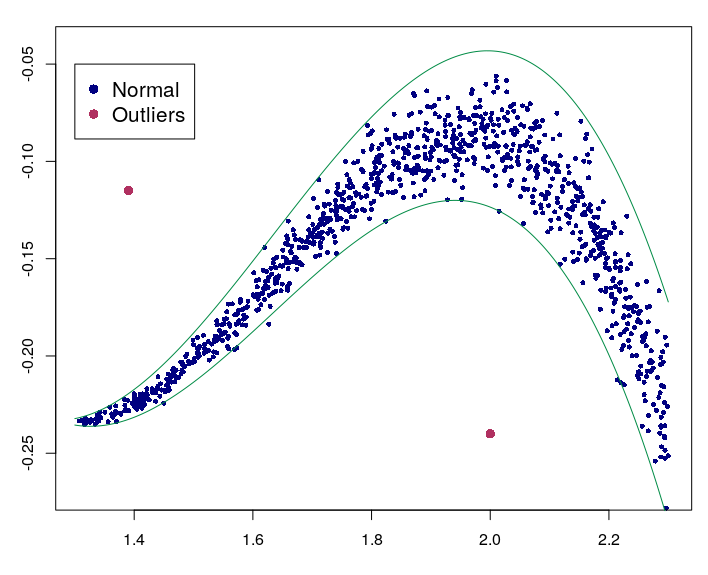
\includegraphics[width=\textwidth]{images/outlier_mine.png}
\caption{}
\end{subfigure}
\begin{subfigure}[b]{0.45\textwidth}
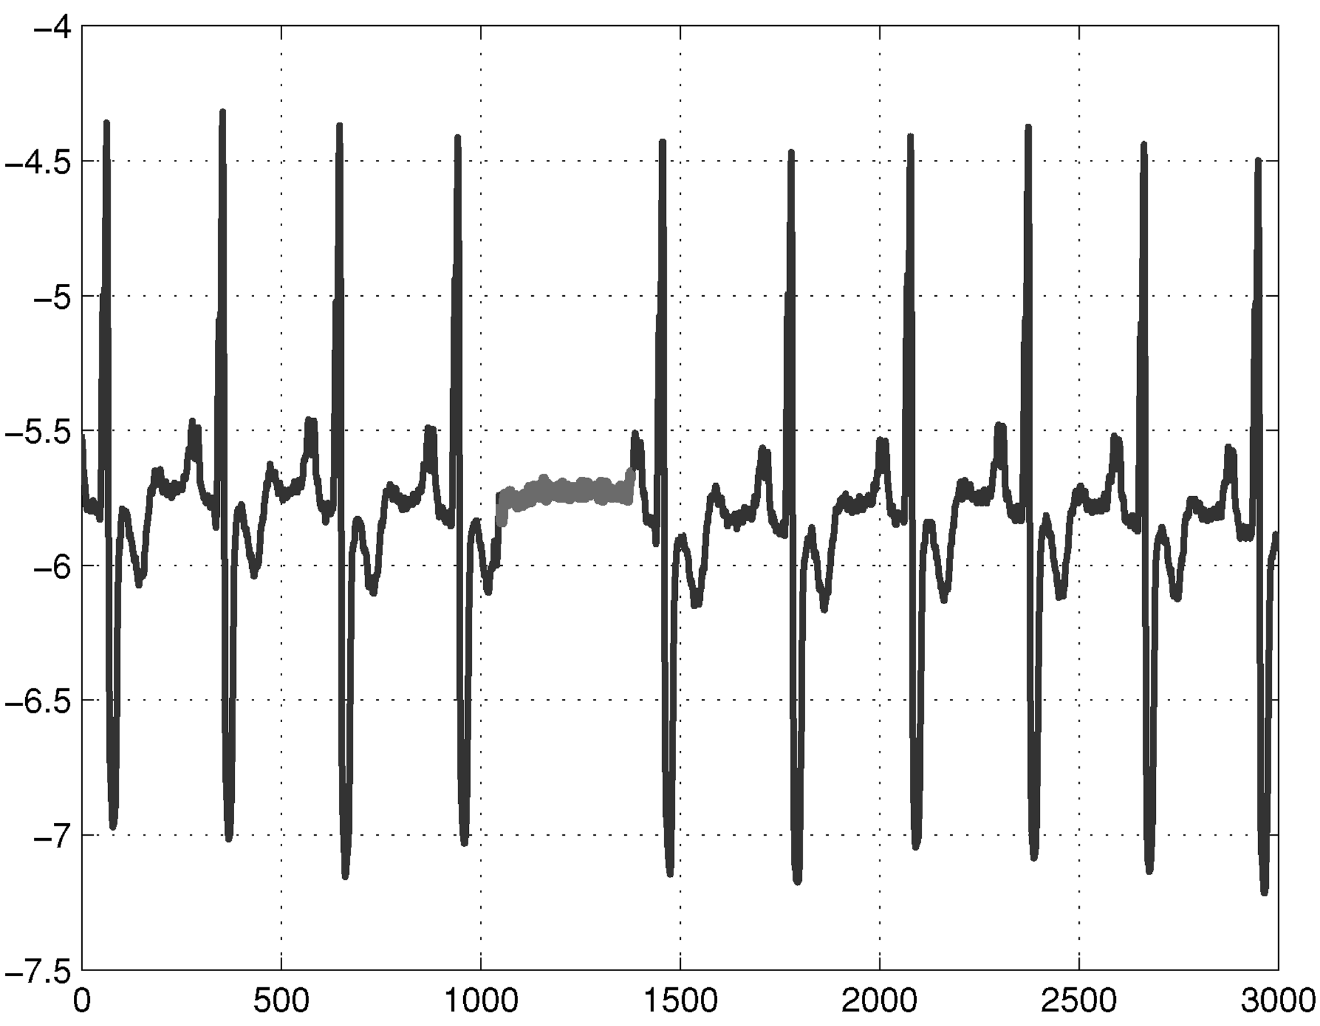
\includegraphics[width=\textwidth]{images/Atrial_Premature_Contraction.png}
\caption{}
\end{subfigure}
\caption{The left plot (a) depicts simple anomalies that deviate in distance from regular data. The right plot (b) shows a contextual anomaly where a group of data instances do not follow a repeating timely behaviour with respect to all other data points (corresponding to an \textit{Atrial Premature Contraction}, taken from \cite{chandola_anomaly_2009})}
\end{figure}

Anomaly detection has found wide application in areas where stability of  critical systems or detection of their abuse is crucial. Examples of these include engine-fault detection in wind-turbines, fraud detection for credit cards. The assumption here is that the modelled system, such as the sensor-data stream of an engine or the buying behaviour of a customer, remains stable and generates consistent data. Detected anomalies in new observations then indicate potential fault or abuse in this system. Obviously, it is not inherently clear that every abuse or fault generates data that differs from normal data. Therefore, it is important to choose data sources are able to reflect the unique nature of a particular system.

\subsubsection{Anomaly detection and NIDS}

Similar to the above described examples, anomaly detection has been applied to network security since the late 90's in order to assist IDSs, with the behaviour of network computers being quantified in the form of events logs capturing network traffic, system calls, etc. The basic approach is to use collected training logs to infer a model of trustworthy activity, and then compare new behaviour against this model. Again, the assumption is that unauthorized and malicious activity will correspond to behaviour that differs from trustworthy one. As an example, an anomalous network traffic pattern in a involving unusual connection pairs could
signify that a hacked computer is extracting or sending out sensitive data to an unauthorized destination.

\textcolor{red}{Insert stuff about NIDS and anomaly detection, drill down on network traffic, maybe talk about technical structure, how training data is gathered, then trained, collection of the traffic, possible anomalies in training data etc, scarcity of datasets. Talk about how anomaly detection should be able to find new attacks compared to signature based approaches}.

\subsubsection{Literature Summary and identified gaps}


Network traffic can be processed into data features of very different nature. Consequently, approaches to apply anomaly detection in network security vary significantly in their scope and methodology. Individual 


Although commercial intrusion detection systems still relies predominantly on \textit{Signature-based} methods, anomaly detection is more and more used  \textcolor{red}{examples}


I provide a detailed analysis of the most important techniques and approaches in my literature review, which can be found in Section \ref{litreview}. 


\subsection{Gaps}

As pointed out above, anomaly detection techniques currently perform best in the detection of attacks of larger volume, such as \textit{DoS attacks} or \textit{Port Scans}, and currently are the most common application in commercial IDS systems \textcolor{red}{reference or example of IDS}. In contrast, research in this area has been less convincing in the context of more targeted attacks that consist of only one or a few connections, with \textit{R2L} and \textit{U2R} attacks currently being the least detected attack classes \cite{nisioti2018intrusion}. 

This can in part be explained by a lack of understanding of how these smaller, more point-like attacks differentiate themselves from normal traffic. Attacks using a larger number of connections will inevitably disturb the  distribution of one or multiple measures of the network, such as the byte-throughput or the port entropy \cite{lakhina2005mining}. However, an attacking connection inserting malicious code to gain control over a computer does not necessarily have different external properties\footnote{also caled \textit{connection summaries}} such as length, size, or port number, than the diverse range of normal connections. Yet, most attempts to detect these types of attacks via anomaly detection rely exclusively on sumary properties of individual connections or packets to draw a border between normal and malicious traffic. Only very few approaches try to detect malicious connections as contextual anomalies, i.e. as traffic events that are not necessarily unusual on their own, but deviate from normal traffic in the context of their immediate temporal neighbourhood. More information about this can be found in my literature review in section \ref{litreview} \textcolor{red}{exact chapter reference}. Considering both the lack of literature in this area, this project will lok more at the intrinsic nature of network traffic which is manifested in the \textit{semantic structure} of packet and connection sequences. 

\textcolor{red}{Talk maybe a bit about robustness? but maybe just mention it in the probject proposal}

\chapter{Proposal}

\section{Project aim}

Chen et al. \cite{chen_2016_robust,chen_more_2016} recently demonstrated the effectiveness of state-based software models in the identification of malicious sequences actions in a streamof permission and API calls of Android applications. This usage of semantic features allowed the discovery of new malware instances and improved the overall robustness of the classifier drastically. 

This project will use the idea of semantic software models and apply it to network traffic data. It combine methods from machine learning and state-based software models, to automatically learn precise semantic models of network traffic generated by one or more machines. The semantic features of network traffic are here understood in terms of sequences of packet or connection metadata that correspond to fixed protocols of information exchange. These models together form a collection of normal semantic network behaviour of a network of machines, with malicious traffic being detected in an anomaly detection manner. Furthermore, a main aspect of this project will be to guarantee adaptivity and robustness of learned models to the evolution of software programs and their corresponding traffic. 

The motivation for the use of semantic models in network traffic stems from the fact that current anomaly detection methods perform poorly in the identification of temporally isolated malicious connections, as described above, as their external properties such as size, duration, or direction, do not necessarily deviate from normal traffic. Attacks with traffic that falls into this category often break into a machine by exploiting loopholes in the processing of information of programs, and in one way or the other breaking the \textcolor{red}{insert}. Traffic with malicious intent will therefore likely deviate in its intrinsic structure from benign one, and should be detectable when modelling this structure using semantic models.







 \textcolor{red}{argue what that means, why it is promising, and that is has been done before on system calls and promises better robustness}

\begin{itemize}
\item Goal 1
\item Goal 2
\item ...
\end{itemize}



\section{Work achieved so far}


\subsection{Data analysis, strategy, and gathering useful data sources}

Although this project is motivated by previous successful applications of ML-driven semantic models for anomaly detection, the differences in the type of data used in this project means that different tools and modelling strategies are necessary. Network traffic usually contains more intrinsic variation and noise, with packets potentially being dropped, and data distribution being afffected by the level of network congestion or by varying input parameters. Therefore, significant amount of time has been spent on initial data analysis and reflection on good modelling strategies. 

Key assumption in this project is the following:

\begin{assumption}\label{Ass1}
Application $A$ running on a computer can be seen as a probability distribution $P_A(X)$ generating sequences $X$ of network events, with $X$ behaving as a random variable.
\end{assumption}

\begin{assumption}\label{Ass2}
Two applications $A$ and $B$ usually have different $P_A(X)$ and $P_B(X)$, which is applies especially to malicious applications. A computer running a set $N$ of applications%\footnote{including OS-applications}
generates sequences $X$ of network events with a distribution $P_N(X)=\sum_{n\in N}P_n(X)$. Consequently, a sophisticated and well enough trained anomaly model of a machine's traffic distribution $P_N(X)$ should be able to identify the existence of a new (and potentially malicious) application as traffic that did not originate from the set of existing applications $N$.
\end{assumption}


\subsubsection{Semantic structures and corresponding variations}

Semantic behaviour of a program denotes how it transmits and reacts to information. This is can be observed both on a packet and on a flow level: Programs follow specific protocols on key-exchange etc. when a connection is established or how and with what frequency new bulks of data-packets are pushed, but also react to data retrieved in one connections with new connection requests such as the establishing of a HTTP-connection to an address received by an earlier DNS-request. Variation and noise is introduced in several ways:

\begin{itemize}

\item Varying sizes of data means a varying number and sizes of packets to be transmitted, which can in turn influence the way the receiver responds. Similarly, requested content can be made up of several files of different sizes which are transmitted in a varying number of connections with differing sizes.
\item Encryption can in a similar way introduce variation in packet or connection sizes and numbers.
\item Variation in the computational load or on the network on a computer can translate into varying response times to retreived information or much data is buffered and pushed at once. Similarly, packet loss or deviations from the established protocol by one side usually means that information has to be transmitted again.

\end{itemize}


% data analysis, and appropriate measures to best capture programs distinctinctive signatures. Signatures from Snort have been helpful

\subsubsection{Alan Turing Data Study Group}



\subsection{Ground truth data generation}

Building semantic models of network traffic means to build an understanding how different network interactions can be distinguished via their traffic trace. We want to use ML techniques to automatically extract meaningful sets of sequences that represent these different interactions. In order to ensure that this is actually true, that our extracted models are indeed representing real distinguishable interactions and not just nonsense, we need validation from \textit{ground truth data}. 

Network traffic datasets are already h7ard to obtain due to privacy concerns. However, as  the correspondance between individual network traffic events and their particular purpose are virtually never recorded on a computer, their exist close to zero datasets containing ground truth about the contained events. For that reason, a particular aspect of this project is to generate useful ground truth data with appropriate content myself.

Over the course of the last year, Nikola Pavlov and I developed a framework that generates controlled and isolated network traffic from a variety of applications and tasks. For this, a virtual network was created using the virtualisation programm \textit{Docker}. In this network, two or more parties can communicate as containers,  which are sandboxes containing programs inside a minimal virtualised operating system. The benefit of this design is that individual containers can only communicate with each other via the virtualised network while the host is in complete control of the parallel execution of tasks in multiple containers. In order to capture the traffic, every container in the network was complemented with a \textit{tcpdump}\footnote{A common packet capture utility}-container hooked onto the network interface. The captured traffic can then be labelled according to the particular scenario it was generated by.


\begin{figure}\label{graph}
\centering
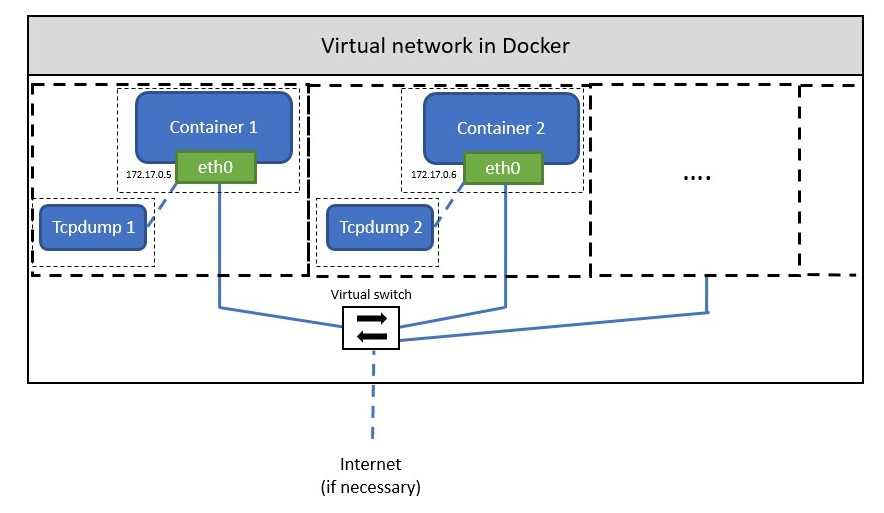
\includegraphics[width=0.7\textwidth]{images/Dockernet.jpg}
\caption{Visualisation of the virtual network in Docker}
\end{figure}

We implemented a variety of network service  scenarios to capture a diverse set of network traffic. Most, but not all, are set up in a server-client manner. Implemented services so far include:

\begin{itemize}
\item A simple icmp ping service.
\item A \textit{nginx} server hosting a html-webpage with a client accessing it, both encrypted and unencrypted. Different client requests are implemented (\textit{Wget} and \textit{Siege}).
\item An \textit{Apache} server hosting the same html-webpage with a client accessing it, also both encrypted and unencrypted. Again, different client requests are implemented (\textit{Wget} and \textit{Siege}).
\item A \textit{Wordpress} server with a corresponding webpage and a client accessing it.
\item Different versions of an ftp server and client.
\item A mail transfer using \textit{mailx}.
\item An ssh-server and client.
\item An \textit{IRC} chat server and two clients.
\item A file synchronisation service with multiple clients.
\item A web-crawler gathering a larger volume of traffic from the internet.
\end{itemize}

For each service, a number of different scenarios are implemented. For example, the ftp client could pull, push, remove, or a combination of all one or multiple files\footnote{that might not exist}, or make directory. Furthermore, randomisation is introduced on parameters like the file-sizes, request times, etc. in order to explore the dimensional variation of the traffic from individual actions.

\textcolor{red}{write about testing the traffic in terms of consistency, problems etc.}.


\textcolor{red}{write about the application of the traffic, how to use it for validation}.


\subsection{Testing first approaches on realistic data}

In the context of the overall research goal of this project, some exploratory work on semantic anomaly detection for network events has been conducted by Marc Sabate, Gudmund Grov, Wei Chen, and David Aspinall. This work uses three different machine learning algorithms\footnote{A Markov Chain model, Finite-State Automata, and a Recurrent Neural Network} from the area of \textit{representation learning} to capture meaningful sequences of \textit{NetFlows} and reflect reoccurring patterns in a model. For that, recorded NetFlows are grouped according to the generating host. Furthermore, in order to filter out sequences of flows that are unrelated to each other, a squence of flows that are close in time is grouped into what is called a \textit{sessions} as an approximation "true relation". Each session then serves as a training or test sequence for a behavioural model. Learned semantic behaviour is reflected through the capability of the model to predict features of the whole session and of other flows in the session from a smaller subset of flows, with more accurate predictions being rewarded in the training process. \textcolor{red}{These features include the network protocol and port and} Sessions which deviate from previously observed behaviour are then predicted poorly by the model and flagged as potentially malicious.

\begin{figure}\label{RNN}
\centering
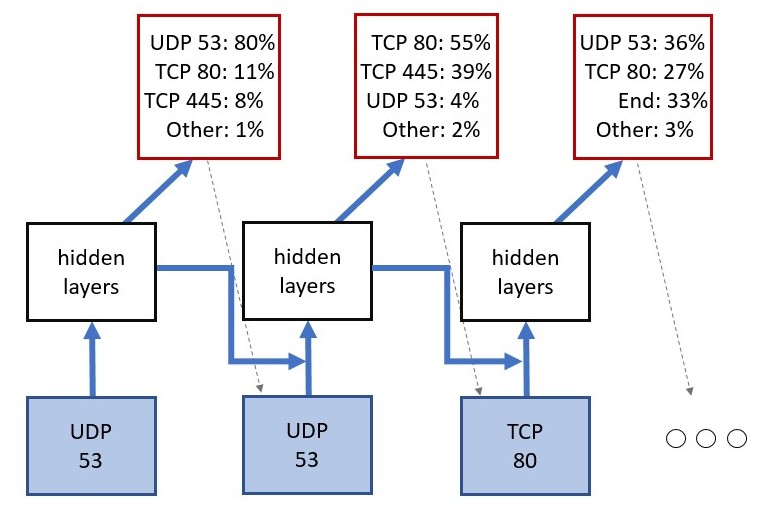
\includegraphics[width=0.7\textwidth]{images/RNN.jpg}
\caption{Visualisation of the RNN-method used}
\end{figure}

\textcolor{red}{maybe write about how these methods are directly relevant for this PhD and could be extended, improved or incorporated}.

The described methods were tested on the CTU-13 dataset \cite{garcia2014empirical}, a laboratory generated dataset available to study botnet detection. The great benefit of this data is the inclusion of both benign background traffic, on which the models were trained, and malicious traffic used to test their detection capabilities, and the availability of corresponding labels. Furthermore, it consists of more than ten million flows on multiple machines, thus containing reasonably much variation for testing purposes.

Anomaly-based methods in intrusion detection are often criticised for working only in controlled environments while failing in the real world. To counter this criticism, it is crucial to provide evidence of success on sufficient data gathered under realistic conditions. For the CTU-13 dataset, the generation of both types of traffic was done in a controlled laboratory environment, making it a so called "synthetic" dataset. This does not necessarily mean that it does not reflect realistic behaviour, however there is no guarantee that it contains all variations encountered in an operational environment. 

\textcolor{red}{As the developed methods are a good foundation to build this project upon}, David Aspinall and I agreed that I should apply the same methods on a real-world datasets that I already worked on during my Master's degree to bolster their results and \textcolor{red}{another justification that this is relevent to my project because of the closeness of the methods}. 

\textcolor{red}{write about LANL and UGR when you are done}

\section{Project specific objectives}


\subsection{Learning representations of connection/protocol behaviour}


NDFA with similarity measure and state merging


RNN approach or Autoencoder

\subsection{Improving current methods}

Using more features

Using extracted features from the connection

Let above mentioned methods provide semantic understanding of connections to form groups, and then give the detected group as an input feature to the methods. That way, specific tasks performed in a connection can be identified and given as input to methods looking at connection sequences



\subsection{Testing}

packet capture dataset, validating with likelihood fit and further validation if captured sequences meaningful with traffic generation tool


\appendix
% appendices come here
\chapter{}
\section{Literature Review}\label{litreview}

%\addcontentsline{toc}{chapter}{Bibliography}
\bibliographystyle{abbrv}
\bibliography{refs}

\end{document}